\subsubsection{Total number of messages sent}\label{subsubsec:hd2krmessages}

This is an indication of the energy efficiency of the entire network.

The maximum number of copies is the dominant factor (\(85.98\%\)), as expected.
Also the broadcast radius \(R\) and its combination with the maximum
number of copies have a valuable impact on this index. The unexplained variation
is very low (\(0.53\%\)).

In \figref{subfig:hdperfmessagesm} we see that the total number of messages sent
decreases with an lower value of the \code{maxCopies} parameter, as expected.
We note that with \(m\!=\!6\) we get that nearly all the users of the network
relay the message. In \figref{subfig:hdperfmessagesR} we can see that less
messages are sent if an higher broadcast radius is used when \(m\!=\!2\). So,
with a low \(m\), we can further decrease the total number of messages sent by
increasing \(R\). Of course increasing the broadcast radius is not good for our
purpose to optimize the energy efficiency of the network, but as we can see from
\figref{subfig:hdperfmessagesT}, the same consideration made for \(R\) are also
valid for the hear window size \(T\). We perhaps expect \(T\) to hugely affect
the total broadcast time, so the selection of the factor \(T\) is a trade-off
between the energy efficiency and the total broadcast time.

\begin{figure}[htb]
	\centering
	\begin{subfigure}[b]{0.38\textwidth}
		\centering
		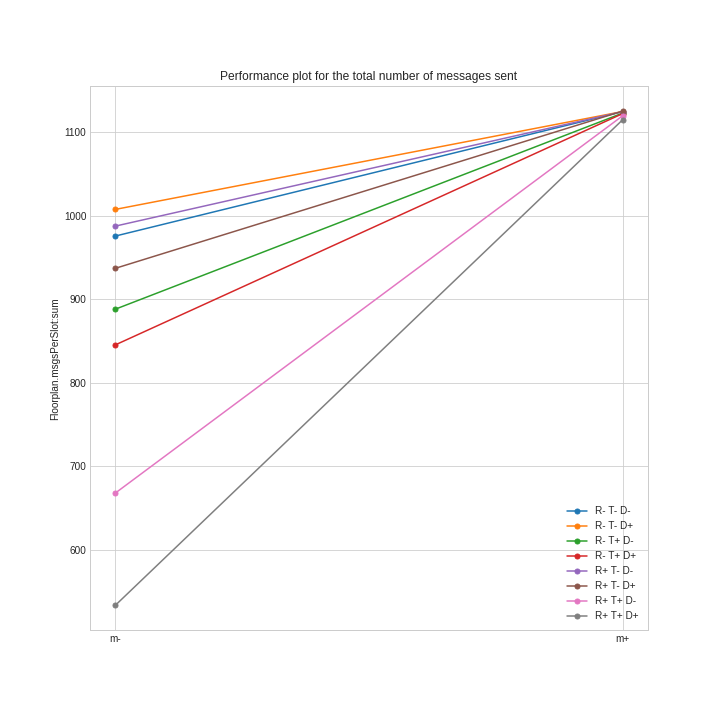
\includegraphics[width=\textwidth]{img/hd/messages-m-perfplot}
		\caption{When the maximum number of copies is reduced the total
		number of messages sent decreases}\label{subfig:hdperfmessagesm}
	\end{subfigure}
	\begin{subfigure}[b]{0.38\textwidth}
		\centering
		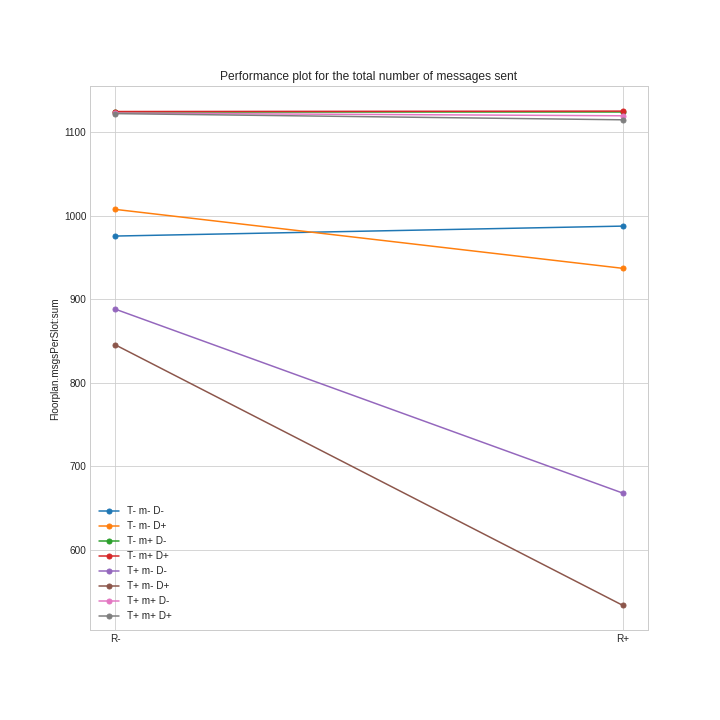
\includegraphics[width=\textwidth]{img/hd/messages-R-perfplot}
		\caption{Increase the broadcast radius when \(m\) is low to
		reduce the total number of messages
		sent}\label{subfig:hdperfmessagesR}
	\end{subfigure}\\
	\begin{subfigure}[b]{0.37\textwidth}
		\centering
		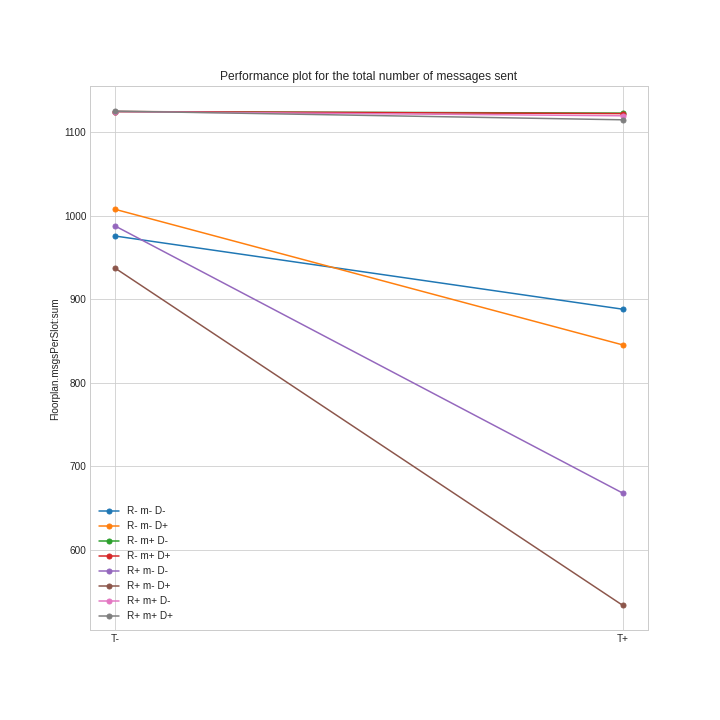
\includegraphics[width=\textwidth]{img/hd/messages-T-perfplot}
		\caption{Increase the size of the hear window when \(m\) is low
		to reduce the total number of messages
		sent}\label{subfig:hdperfmessagesT}
	\end{subfigure}
	\caption{Performance plots for the total number of messages
	sent}\label{fig:hdperfmessages}
\end{figure}
